\documentclass{article}
\usepackage{tikz}
\usepackage{amsmath}

\begin{document}

\begin{center}
    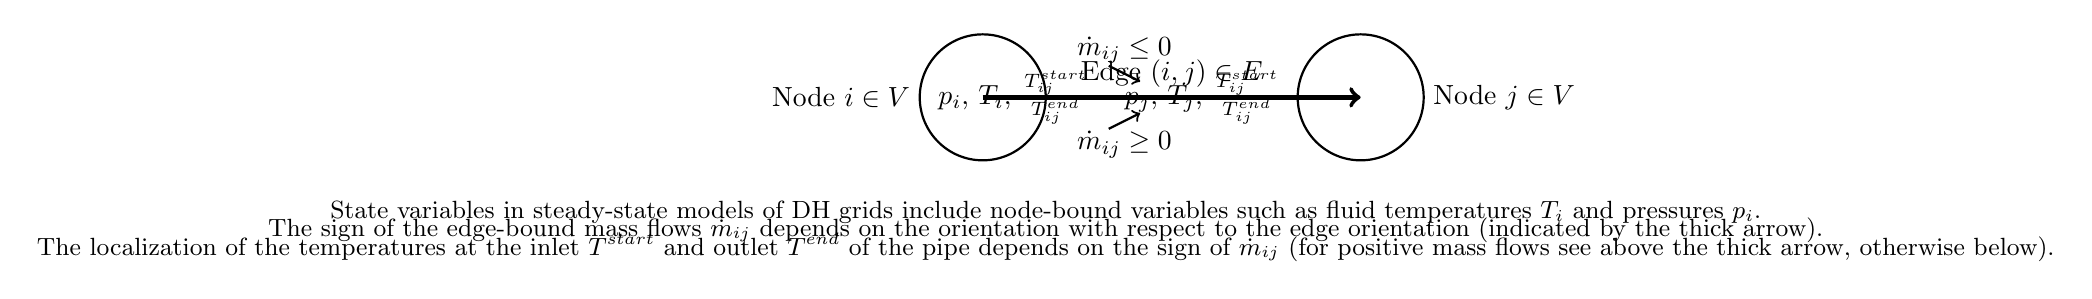
\begin{tikzpicture}[scale=0.8]
        % Nodes
        \draw[thick] (-3,0) circle [radius=1];
        \node[left] at (-4,0) {Node $i \in V$};
        \node at (-2.5,0) {$p_i$, $T_i$, $\frac{T_{ij}^{start}}{T_{ij}^{end}}$};
        \draw[thick] (3,0) circle [radius=1];
        \node[right] at (4,0) {Node $j \in V$};
        \node at (0.5,0) {$p_j$, $T_j$, $\frac{T_{ij}^{start}}{T_{ij}^{end}}$};

        % Edge
        \draw[ultra thick,->] (-3,0) -- (3,0);
        \node[above] at (0,0) {Edge $(i,j) \in E$};
        
        % Sign conditions
        \draw[thick,->] (-1,-0.5) -- (-0.5,-0.25);
        \node at (-0.75,-0.75) {$\dot{m}_{ij} \geq 0$};
        \draw[thick,->] (-1,0.5) -- (-0.5,0.25);
        \node at (-0.75,0.75) {$\dot{m}_{ij} \leq 0$};
        
        % Text for steady-state model
        \node[below] at (-2,-1.5) {\small State variables in steady-state models of DH grids include node-bound variables such as fluid temperatures $T_i$ and pressures $p_i$.};
        \node[below] at (-2,-1.75) {\small The sign of the edge-bound mass flows $\dot{m}_{ij}$ depends on the orientation with respect to the edge orientation (indicated by the thick arrow).};
        \node[below] at (-2,-2) {\small The localization of the temperatures at the inlet $T_{}^{start}$ and outlet $T_{}^{end}$ of the pipe depends on the sign of $\dot{m}_{ij}$ (for positive mass flows see above the thick arrow, otherwise below).};
    \end{tikzpicture}
\end{center}

\end{document}